% Standalone preview: Four Retrieval Motifs
% Compile: pdflatex fig_motifs.tex
\documentclass[tikz,border=14pt]{standalone}
\usepackage{tikz}
\usetikzlibrary{arrows.meta,positioning,backgrounds,fit,decorations.pathreplacing}

% ── Colours ──────────────────────────────────────────────────────────────────
\definecolor{anchorblue}{RGB}{37,99,235}
\definecolor{bridgeorange}{RGB}{234,88,12}
\definecolor{steingreen}{RGB}{22,163,74}
\definecolor{pprpurple}{RGB}{124,58,237}
\definecolor{nodegray}{RGB}{156,163,175}

\begin{document}
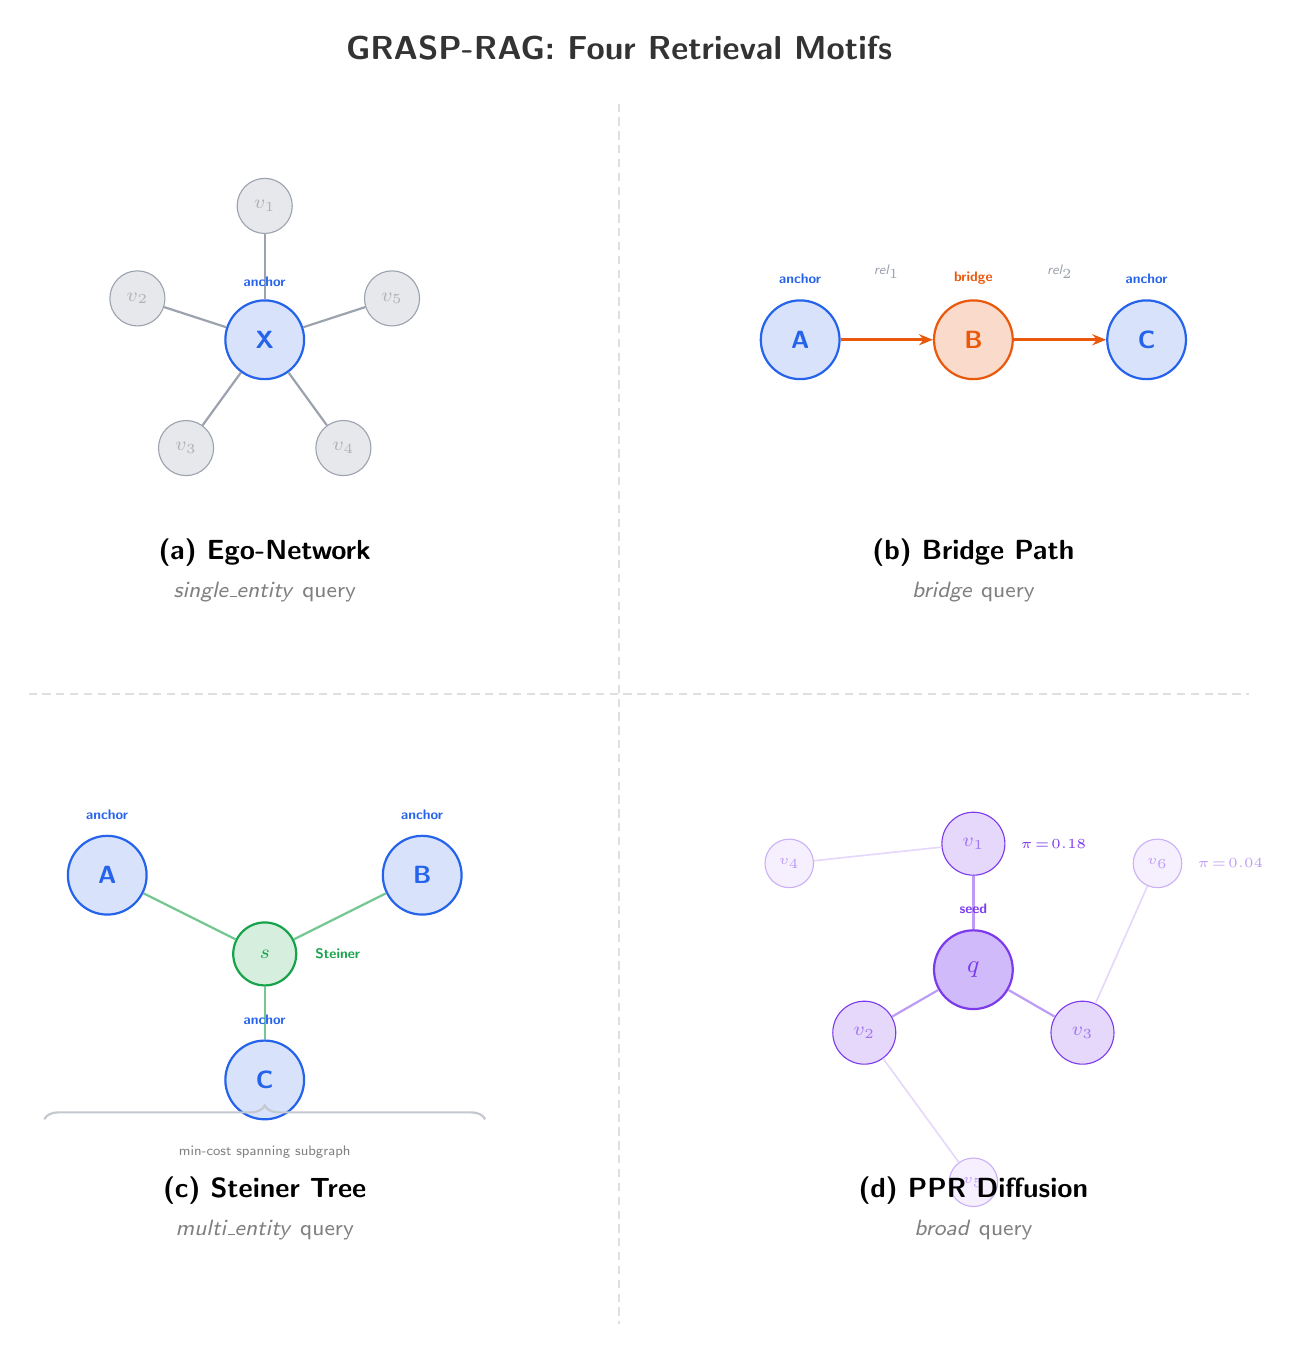
\begin{tikzpicture}[
  % ── node styles ─────────────────────────────────────────────────────
  anode/.style  = {circle, draw=anchorblue,   fill=anchorblue!18,
                   minimum size=10mm, font=\small\bfseries\sffamily,
                   thick, text=anchorblue},
  rnode/.style  = {circle, draw=nodegray,     fill=nodegray!25,
                   minimum size=7mm,  font=\scriptsize\sffamily,
                   text=gray!60},
  bnode/.style  = {circle, draw=bridgeorange, fill=bridgeorange!22,
                   minimum size=10mm, font=\small\bfseries\sffamily,
                   thick, text=bridgeorange},
  snode/.style  = {circle, draw=steingreen,   fill=steingreen!18,
                   minimum size=8mm,  font=\scriptsize\sffamily,
                   thick, text=steingreen},
  pnodeA/.style = {circle, draw=pprpurple,    fill=pprpurple!35,
                   minimum size=10mm, font=\small\bfseries\sffamily,
                   thick, text=pprpurple},
  pnodeB/.style = {circle, draw=pprpurple,    fill=pprpurple!20,
                   minimum size=8mm,  font=\scriptsize\sffamily,
                   text=pprpurple!70},
  pnodeC/.style = {circle, draw=pprpurple!40, fill=pprpurple!8,
                   minimum size=6mm,  font=\tiny\sffamily,
                   text=pprpurple!50},
  % ── edge styles ─────────────────────────────────────────────────────
  eline/.style  = {draw=nodegray,       thick},
  bline/.style  = {draw=bridgeorange,   very thick,
                   -{Stealth[length=5pt,width=4pt]}},
  pline/.style  = {draw=pprpurple!50,   thick},
  pfade/.style  = {draw=pprpurple!20,   semithick},
  % ── label styles ────────────────────────────────────────────────────
  mtitle/.style = {font=\normalsize\bfseries\sffamily, text=black},
  msub/.style   = {font=\footnotesize\sffamily, text=gray},
  tag/.style    = {font=\tiny\sffamily},
]

%% ══════════════════════════════════════════════════════════════════════
%%  (a)  EGO-NETWORK  —  single_entity
%% ══════════════════════════════════════════════════════════════════════
\begin{scope}[shift={(0,0)}]
  \node[anode] (c)  at (0,0)          {X};
  \node[rnode] (r1) at (90:1.7)       {$v_1$};
  \node[rnode] (r2) at (90+72:1.7)    {$v_2$};
  \node[rnode] (r3) at (90+144:1.7)   {$v_3$};
  \node[rnode] (r4) at (90+216:1.7)   {$v_4$};
  \node[rnode] (r5) at (90+288:1.7)   {$v_5$};
  \foreach \n in {r1,r2,r3,r4,r5} \draw[eline] (c) -- (\n);
  % anchor badge
  \node[tag, text=anchorblue, above=1pt of c] {\textbf{anchor}};
  % title
  \node[mtitle] at (0,-2.7) {(a) Ego-Network};
  \node[msub]   at (0,-3.2) {\textit{single\_entity} query};
\end{scope}

%% ══════════════════════════════════════════════════════════════════════
%%  (b)  BRIDGE PATH  —  bridge
%% ══════════════════════════════════════════════════════════════════════
\begin{scope}[shift={(9,0)}]
  \node[anode] (src) at (-2.2, 0) {A};
  \node[bnode] (br)  at ( 0,   0) {B};
  \node[anode] (tgt) at ( 2.2, 0) {C};
  \draw[bline] (src) -- (br);
  \draw[bline] (br)  -- (tgt);
  % edge keyword labels
  \node[tag, text=nodegray, above=4pt of br, xshift=-1.1cm]
        {\textit{rel$_1$}};
  \node[tag, text=nodegray, above=4pt of br, xshift= 1.1cm]
        {\textit{rel$_2$}};
  % badges
  \node[tag, text=anchorblue,    above=2pt of src] {\textbf{anchor}};
  \node[tag, text=bridgeorange,  above=2pt of br]  {\textbf{bridge}};
  \node[tag, text=anchorblue,    above=2pt of tgt] {\textbf{anchor}};
  % title
  \node[mtitle] at (0,-2.7) {(b) Bridge Path};
  \node[msub]   at (0,-3.2) {\textit{bridge} query};
\end{scope}

%% ══════════════════════════════════════════════════════════════════════
%%  (c)  STEINER TREE  —  multi_entity
%% ══════════════════════════════════════════════════════════════════════
\begin{scope}[shift={(0,-8)}]
  % Three anchor nodes
  \node[anode] (a1) at (-2,  1.2) {A};
  \node[anode] (a2) at ( 2,  1.2) {B};
  \node[anode] (a3) at ( 0, -1.4) {C};
  % Steiner intermediate node
  \node[snode] (s1) at ( 0,  0.2) {$s$};
  % Steiner edges
  \draw[eline, draw=steingreen!60, thick] (a1) -- (s1);
  \draw[eline, draw=steingreen!60, thick] (a2) -- (s1);
  \draw[eline, draw=steingreen!60, thick] (a3) -- (s1);
  % badges
  \foreach \n/\l in {a1/anchor, a2/anchor, a3/anchor}
    \node[tag, text=anchorblue, above=2pt of \n] {\textbf{\l}};
  \node[tag, text=steingreen, right=3pt of s1] {\textbf{Steiner}};
  % brace label
  \draw[decorate, decoration={brace,amplitude=5pt},
        draw=nodegray!60, thick]
    (-2.8,-1.9) -- (2.8,-1.9)
    node[midway, below=6pt, font=\tiny\sffamily, text=gray]
         {min-cost spanning subgraph};
  % title
  \node[mtitle] at (0,-2.8) {(c) Steiner Tree};
  \node[msub]   at (0,-3.3) {\textit{multi\_entity} query};
\end{scope}

%% ══════════════════════════════════════════════════════════════════════
%%  (d)  PPR DIFFUSION  —  broad
%% ══════════════════════════════════════════════════════════════════════
\begin{scope}[shift={(9,-8)}]
  % Seed node
  \node[pnodeA] (seed) at (0,0) {$q$};
  % Ring 1 — high PPR
  \node[pnodeB] (p1) at ( 90:1.6) {$v_1$};
  \node[pnodeB] (p2) at (210:1.6) {$v_2$};
  \node[pnodeB] (p3) at (330:1.6) {$v_3$};
  % Ring 2 — low PPR
  \node[pnodeC] (p4) at (150:2.7) {$v_4$};
  \node[pnodeC] (p5) at (270:2.7) {$v_5$};
  \node[pnodeC] (p6) at ( 30:2.7) {$v_6$};
  % Edges ring-0 to ring-1
  \draw[pline] (seed) -- (p1);
  \draw[pline] (seed) -- (p2);
  \draw[pline] (seed) -- (p3);
  % Edges ring-1 to ring-2
  \draw[pfade] (p1) -- (p4);
  \draw[pfade] (p2) -- (p5);
  \draw[pfade] (p3) -- (p6);
  % PPR score annotations
  \node[tag, text=pprpurple,   right=2pt of p1] {$\pi\!=\!0.18$};
  \node[tag, text=pprpurple!50, right=2pt of p6] {$\pi\!=\!0.04$};
  % badge
  \node[tag, text=pprpurple, above=2pt of seed] {\textbf{seed}};
  % title
  \node[mtitle] at (0,-2.8) {(d) PPR Diffusion};
  \node[msub]   at (0,-3.3) {\textit{broad} query};
\end{scope}

%% ══════════════════════════════════════════════════════════════════════
%%  Dividers
%% ══════════════════════════════════════════════════════════════════════
\draw[gray!25, densely dashed, line width=0.6pt]
  (4.5, 3) -- (4.5,-12.5);
\draw[gray!25, densely dashed, line width=0.6pt]
  (-3, -4.5) -- (12.5,-4.5);

%% ══════════════════════════════════════════════════════════════════════
%%  Overall title
%% ══════════════════════════════════════════════════════════════════════
\node[font=\large\bfseries\sffamily, text=black!80]
  at (4.5, 3.7) {GRASP-RAG: Four Retrieval Motifs};

\end{tikzpicture}
\end{document}
